\chapter{序論}
\section{背景}
農業従事者の高齢化や後継者不足などによって作業者の負担が増加しているため, 作業の機械化や自動化が期待されている. 
特に生産の場ではない畦道での草刈り作業は小型機械を背負うなどして人力での作業が行われており, 雑草の成長が著しく高温である夏季に繰り返し行わなければならない重労働である. 
また農地内での荷物の運搬を人力で行う際には農作業一輪車が使われており, 畦道などの細く不安定な道での重量物の運搬は容易とは言い難い. 
これらのように農業には生産活動以外にも従事者の負担となる作業も多くある.  

そのなかで作業負担を減らすための手段のひとつとして移動ロボットの活用が考えられる. 
移動ロボットが自動で畦道を走行することにより荷物の運搬や草刈り作業を自動化をできることや, 
走行する際に畦道上の雑草に対して上から圧力を加えることで雑草の成長の抑制も期待できる\cite{稲垣栄洋2017踏圧処理が畦畔雑草植生に及ぼす影響}. 
このように移動ロボットが畦道を走行することによって様々な作業負担を減らすことが可能であると考えた. 

しかし, これらの例を実現するには様々な問題がある.  
例えば畦道と水田には明確な境界がないために検出が困難であり, 走行箇所である畦道から外れてしまう恐れがあることや, 
傾斜から水田に滑り落ちる可能性があるなどの問題があげられる. 
そのため移動ロボットが自動で畦道を走行するためには, 安全に走行することができる路面を検出する必要がある.


%@@@草ぼうぼうのあぜみちの写真とかがあると説得力出ますね. 

\section{従来研究}

%@@@全体的に読点が少ないような気がします. 
畦道と水田の間には白線や縁石などのような目印となる物がなく, 土を盛り上げているだけであり境界が曖昧である. 
そのため自動運転などに用いられている白線などを基準とした走行箇所の選定を行うことができない. 
そこで畦道上では路面の状態をニューラルネットワークを用いて判別し, 
走行箇所の選定を行う研究\cite{長橋孝哉2019ニューラルネットワークを用いた畦道の雑草検出に関する研究}がある.  
%%%%「路面の検出に関しては」はざっくりしすぎ. 

この研究では畦道上の雑草領域を走行箇所としており, 
単眼カメラから得た画像をR, G, BとH, S, Vの平均値と分散を特徴量としてニューラルネットワークを用いて学習し, 
入力された画像を格子状に二つのクラスに分類している. 
雑草領域の分類に成功しているが色の類似した物に対しての誤認識が起きており, 図 1.2のような畦道では走行箇所ではない水田への誤認識が予想される. 

\begin{figure}[htbp]
\begin{center}
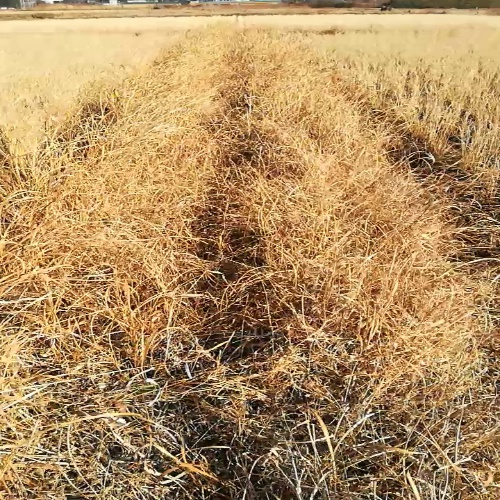
\includegraphics[width=100mm]{figs/fig2.jpg}
\caption{}
\end{center}
\end{figure}

%@@@!!!!!!!!!!!!!!!だから何???????次のパートにつながらない. 

%畦道における移動ロボットの研究例としては人間がリモコンを用いて操作するラジコン型ロボットや, 道幅や傾斜がある程度整備された環境内での自動走行が可能なロボットがある. 
%これらのロボットを使用することにより人力で行っていた作業の負担を軽減することができるが, 環境の整備などの新たな作業が増える. 
\section{研究の目的}
走行箇所である畦道から外れて走行することを防ぐために画像中から畦道領域を取得
水田への落下を防ぐために畦道領域の取得と路面状況の評価を併用し走行可能な路面を検出すること

%@@@ちゃんと段落分けしましょうね. 参考: https://b.ueda.tech/?post=02586

% dvipdfmxとhereのテスト
%\begin{figure}[H]
%	\begin{center}
%		
\includegraphics[width=1.0\linewidth]{../zero.png}
%		\caption{}
%		\label{fig:}
%	\end{center}
%\end{figure}
%
